% Options for packages loaded elsewhere
\PassOptionsToPackage{unicode}{hyperref}
\PassOptionsToPackage{hyphens}{url}
%
\documentclass[
]{article}
\title{class09}
\author{Vince (PID: A15422556)}
\date{2/15/2022}

\usepackage{amsmath,amssymb}
\usepackage{lmodern}
\usepackage{iftex}
\ifPDFTeX
  \usepackage[T1]{fontenc}
  \usepackage[utf8]{inputenc}
  \usepackage{textcomp} % provide euro and other symbols
\else % if luatex or xetex
  \usepackage{unicode-math}
  \defaultfontfeatures{Scale=MatchLowercase}
  \defaultfontfeatures[\rmfamily]{Ligatures=TeX,Scale=1}
\fi
% Use upquote if available, for straight quotes in verbatim environments
\IfFileExists{upquote.sty}{\usepackage{upquote}}{}
\IfFileExists{microtype.sty}{% use microtype if available
  \usepackage[]{microtype}
  \UseMicrotypeSet[protrusion]{basicmath} % disable protrusion for tt fonts
}{}
\makeatletter
\@ifundefined{KOMAClassName}{% if non-KOMA class
  \IfFileExists{parskip.sty}{%
    \usepackage{parskip}
  }{% else
    \setlength{\parindent}{0pt}
    \setlength{\parskip}{6pt plus 2pt minus 1pt}}
}{% if KOMA class
  \KOMAoptions{parskip=half}}
\makeatother
\usepackage{xcolor}
\IfFileExists{xurl.sty}{\usepackage{xurl}}{} % add URL line breaks if available
\IfFileExists{bookmark.sty}{\usepackage{bookmark}}{\usepackage{hyperref}}
\hypersetup{
  pdftitle={class09},
  pdfauthor={Vince (PID: A15422556)},
  hidelinks,
  pdfcreator={LaTeX via pandoc}}
\urlstyle{same} % disable monospaced font for URLs
\usepackage[margin=1in]{geometry}
\usepackage{color}
\usepackage{fancyvrb}
\newcommand{\VerbBar}{|}
\newcommand{\VERB}{\Verb[commandchars=\\\{\}]}
\DefineVerbatimEnvironment{Highlighting}{Verbatim}{commandchars=\\\{\}}
% Add ',fontsize=\small' for more characters per line
\usepackage{framed}
\definecolor{shadecolor}{RGB}{248,248,248}
\newenvironment{Shaded}{\begin{snugshade}}{\end{snugshade}}
\newcommand{\AlertTok}[1]{\textcolor[rgb]{0.94,0.16,0.16}{#1}}
\newcommand{\AnnotationTok}[1]{\textcolor[rgb]{0.56,0.35,0.01}{\textbf{\textit{#1}}}}
\newcommand{\AttributeTok}[1]{\textcolor[rgb]{0.77,0.63,0.00}{#1}}
\newcommand{\BaseNTok}[1]{\textcolor[rgb]{0.00,0.00,0.81}{#1}}
\newcommand{\BuiltInTok}[1]{#1}
\newcommand{\CharTok}[1]{\textcolor[rgb]{0.31,0.60,0.02}{#1}}
\newcommand{\CommentTok}[1]{\textcolor[rgb]{0.56,0.35,0.01}{\textit{#1}}}
\newcommand{\CommentVarTok}[1]{\textcolor[rgb]{0.56,0.35,0.01}{\textbf{\textit{#1}}}}
\newcommand{\ConstantTok}[1]{\textcolor[rgb]{0.00,0.00,0.00}{#1}}
\newcommand{\ControlFlowTok}[1]{\textcolor[rgb]{0.13,0.29,0.53}{\textbf{#1}}}
\newcommand{\DataTypeTok}[1]{\textcolor[rgb]{0.13,0.29,0.53}{#1}}
\newcommand{\DecValTok}[1]{\textcolor[rgb]{0.00,0.00,0.81}{#1}}
\newcommand{\DocumentationTok}[1]{\textcolor[rgb]{0.56,0.35,0.01}{\textbf{\textit{#1}}}}
\newcommand{\ErrorTok}[1]{\textcolor[rgb]{0.64,0.00,0.00}{\textbf{#1}}}
\newcommand{\ExtensionTok}[1]{#1}
\newcommand{\FloatTok}[1]{\textcolor[rgb]{0.00,0.00,0.81}{#1}}
\newcommand{\FunctionTok}[1]{\textcolor[rgb]{0.00,0.00,0.00}{#1}}
\newcommand{\ImportTok}[1]{#1}
\newcommand{\InformationTok}[1]{\textcolor[rgb]{0.56,0.35,0.01}{\textbf{\textit{#1}}}}
\newcommand{\KeywordTok}[1]{\textcolor[rgb]{0.13,0.29,0.53}{\textbf{#1}}}
\newcommand{\NormalTok}[1]{#1}
\newcommand{\OperatorTok}[1]{\textcolor[rgb]{0.81,0.36,0.00}{\textbf{#1}}}
\newcommand{\OtherTok}[1]{\textcolor[rgb]{0.56,0.35,0.01}{#1}}
\newcommand{\PreprocessorTok}[1]{\textcolor[rgb]{0.56,0.35,0.01}{\textit{#1}}}
\newcommand{\RegionMarkerTok}[1]{#1}
\newcommand{\SpecialCharTok}[1]{\textcolor[rgb]{0.00,0.00,0.00}{#1}}
\newcommand{\SpecialStringTok}[1]{\textcolor[rgb]{0.31,0.60,0.02}{#1}}
\newcommand{\StringTok}[1]{\textcolor[rgb]{0.31,0.60,0.02}{#1}}
\newcommand{\VariableTok}[1]{\textcolor[rgb]{0.00,0.00,0.00}{#1}}
\newcommand{\VerbatimStringTok}[1]{\textcolor[rgb]{0.31,0.60,0.02}{#1}}
\newcommand{\WarningTok}[1]{\textcolor[rgb]{0.56,0.35,0.01}{\textbf{\textit{#1}}}}
\usepackage{graphicx}
\makeatletter
\def\maxwidth{\ifdim\Gin@nat@width>\linewidth\linewidth\else\Gin@nat@width\fi}
\def\maxheight{\ifdim\Gin@nat@height>\textheight\textheight\else\Gin@nat@height\fi}
\makeatother
% Scale images if necessary, so that they will not overflow the page
% margins by default, and it is still possible to overwrite the defaults
% using explicit options in \includegraphics[width, height, ...]{}
\setkeys{Gin}{width=\maxwidth,height=\maxheight,keepaspectratio}
% Set default figure placement to htbp
\makeatletter
\def\fps@figure{htbp}
\makeatother
\setlength{\emergencystretch}{3em} % prevent overfull lines
\providecommand{\tightlist}{%
  \setlength{\itemsep}{0pt}\setlength{\parskip}{0pt}}
\setcounter{secnumdepth}{-\maxdimen} % remove section numbering
\ifLuaTeX
  \usepackage{selnolig}  % disable illegal ligatures
\fi

\begin{document}
\maketitle

\hypertarget{the-pdb-database}{%
\subsection{The PDB Database}\label{the-pdb-database}}

The PDB is the main repository for 3d structure data of biomolecules.
Here we explore its composition.

\begin{Shaded}
\begin{Highlighting}[]
\NormalTok{pdbData }\OtherTok{\textless{}{-}} \FunctionTok{read.csv}\NormalTok{(}\StringTok{"Data Export Summary.csv"}\NormalTok{, }\AttributeTok{row.names=}\DecValTok{1}\NormalTok{)}
\NormalTok{pdbData}
\end{Highlighting}
\end{Shaded}

\begin{verbatim}
##                          X.ray   NMR   EM Multiple.methods Neutron Other  Total
## Protein (only)          144301 11877 6676              182      70    32 163138
## Protein/Oligosaccharide   8528    31 1116                5       0     0   9680
## Protein/NA                7617   274 2153                3       0     0  10047
## Nucleic acid (only)       2393  1398   61                8       2     1   3863
## Other                      150    31    3                0       0     0    184
## Oligosaccharide (only)      11     6    0                1       0     4     22
\end{verbatim}

\begin{quote}
Q1: What percentage of structures in the PDB are solved by X-Ray and
Electron Microscopy. 87.197\% of structures are solved by X-ray and
5.354\% of structures are solved by EM.
\end{quote}

\begin{Shaded}
\begin{Highlighting}[]
\NormalTok{tot.method }\OtherTok{\textless{}{-}} \FunctionTok{colSums}\NormalTok{(pdbData)}
\FunctionTok{round}\NormalTok{(tot.method}\SpecialCharTok{/}\NormalTok{tot.method[}\StringTok{"Total"}\NormalTok{] }\SpecialCharTok{*} \DecValTok{100}\NormalTok{, }\DecValTok{3}\NormalTok{)}
\end{Highlighting}
\end{Shaded}

\begin{verbatim}
##            X.ray              NMR               EM Multiple.methods 
##           87.197            7.284            5.354            0.106 
##          Neutron            Other            Total 
##            0.039            0.020          100.000
\end{verbatim}

\begin{quote}
Q2: What proportion of structures in the PDB are protein? 87.27
proportion of structures in the PDB are protein.
\end{quote}

\begin{Shaded}
\begin{Highlighting}[]
\NormalTok{ans }\OtherTok{\textless{}{-}}\NormalTok{ pdbData}\SpecialCharTok{$}\NormalTok{Total[}\DecValTok{1}\NormalTok{] }\SpecialCharTok{/} \FunctionTok{sum}\NormalTok{(pdbData}\SpecialCharTok{$}\NormalTok{Total) }\SpecialCharTok{*} \DecValTok{100}
\FunctionTok{round}\NormalTok{(ans, }\DecValTok{3}\NormalTok{)}
\end{Highlighting}
\end{Shaded}

\begin{verbatim}
## [1] 87.27
\end{verbatim}

The answer to this question is 87.27 \% of total structures.

\begin{quote}
Q3: Type HIV in the PDB website search box on the home page and
determine how many HIV-1 protease structures are in the current PDB?
4483 structures.
\end{quote}

\hypertarget{visualizing-the-hiv-1-protease-structure}{%
\subsection{Visualizing the HIV-1 Protease
Structure}\label{visualizing-the-hiv-1-protease-structure}}

\begin{quote}
Q4: Water molecules normally have 3 atoms. Why do we see just one atom
per water molecule in this structure? The hydrogen atom is very small in
comparison to the rest of the molecule.
\end{quote}

\begin{quote}
Q5: There is a conserved water molecule in the binding site. Can you
identify this water molecule? What residue number does this water
molecule have (see note below)? Residue number 308
\end{quote}

VMD generated image of HIV-protease, PDB code: 1hsg

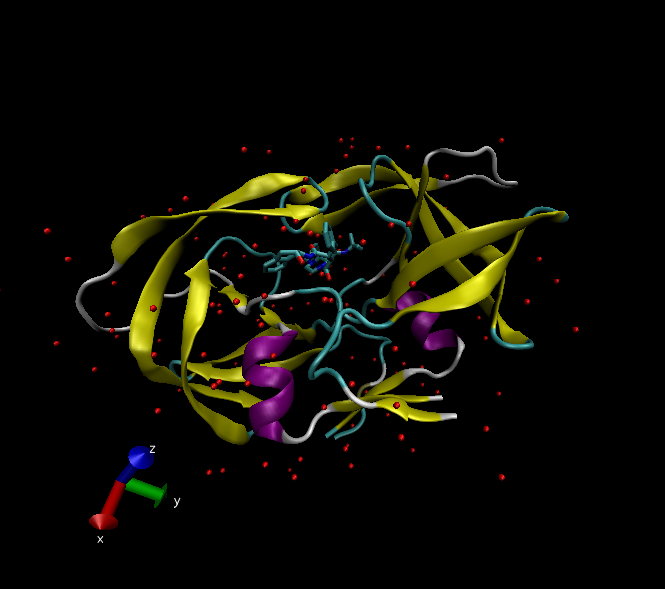
\includegraphics{hiv_image.png}

\hypertarget{sequence-viewer-extension}{%
\subsection{Sequence Viewer Extension}\label{sequence-viewer-extension}}

\begin{quote}
Q6: As you have hopefully observed HIV protease is a homodimer (i.e.~it
is composed of two identical chains). With the aid of the graphic
display and the sequence viewer extension can you identify secondary
structure elements that are likely to only form in the dimer rather than
the monomer? Beta-pleated sheets and alpha helices are likely to form in
the dimer.
\end{quote}

\hypertarget{bio3d-in-r}{%
\subsection{Bio3D in R}\label{bio3d-in-r}}

\begin{Shaded}
\begin{Highlighting}[]
\FunctionTok{library}\NormalTok{(bio3d)}

\NormalTok{pdb }\OtherTok{\textless{}{-}} \FunctionTok{read.pdb}\NormalTok{(}\StringTok{"1hsg"}\NormalTok{)}
\end{Highlighting}
\end{Shaded}

\begin{verbatim}
##   Note: Accessing on-line PDB file
\end{verbatim}

\begin{Shaded}
\begin{Highlighting}[]
\NormalTok{pdb}
\end{Highlighting}
\end{Shaded}

\begin{verbatim}
## 
##  Call:  read.pdb(file = "1hsg")
## 
##    Total Models#: 1
##      Total Atoms#: 1686,  XYZs#: 5058  Chains#: 2  (values: A B)
## 
##      Protein Atoms#: 1514  (residues/Calpha atoms#: 198)
##      Nucleic acid Atoms#: 0  (residues/phosphate atoms#: 0)
## 
##      Non-protein/nucleic Atoms#: 172  (residues: 128)
##      Non-protein/nucleic resid values: [ HOH (127), MK1 (1) ]
## 
##    Protein sequence:
##       PQITLWQRPLVTIKIGGQLKEALLDTGADDTVLEEMSLPGRWKPKMIGGIGGFIKVRQYD
##       QILIEICGHKAIGTVLVGPTPVNIIGRNLLTQIGCTLNFPQITLWQRPLVTIKIGGQLKE
##       ALLDTGADDTVLEEMSLPGRWKPKMIGGIGGFIKVRQYDQILIEICGHKAIGTVLVGPTP
##       VNIIGRNLLTQIGCTLNF
## 
## + attr: atom, xyz, seqres, helix, sheet,
##         calpha, remark, call
\end{verbatim}

\begin{quote}
Q7: How many amino acid residues are there in this pdb object? 198
residues
\end{quote}

\begin{quote}
Q8: Name one of the two non-protein residues? MK1
\end{quote}

\begin{quote}
Q9: How many protein chains are in this structure? 2 protein chains
\end{quote}

\hypertarget{comparative-structure-analysis-of-adenylate-kinase}{%
\subsection{Comparative structure analysis of Adenylate
Kinase}\label{comparative-structure-analysis-of-adenylate-kinase}}

Extract the sequence for ADK

\begin{Shaded}
\begin{Highlighting}[]
\NormalTok{aa }\OtherTok{\textless{}{-}} \FunctionTok{get.seq}\NormalTok{(}\StringTok{"1ake\_A"}\NormalTok{)}
\end{Highlighting}
\end{Shaded}

\begin{verbatim}
## Warning in get.seq("1ake_A"): Removing existing file: seqs.fasta
\end{verbatim}

\begin{verbatim}
## Fetching... Please wait. Done.
\end{verbatim}

\begin{Shaded}
\begin{Highlighting}[]
\NormalTok{aa}
\end{Highlighting}
\end{Shaded}

\begin{verbatim}
##              1        .         .         .         .         .         60 
## pdb|1AKE|A   MRIILLGAPGAGKGTQAQFIMEKYGIPQISTGDMLRAAVKSGSELGKQAKDIMDAGKLVT
##              1        .         .         .         .         .         60 
## 
##             61        .         .         .         .         .         120 
## pdb|1AKE|A   DELVIALVKERIAQEDCRNGFLLDGFPRTIPQADAMKEAGINVDYVLEFDVPDELIVDRI
##             61        .         .         .         .         .         120 
## 
##            121        .         .         .         .         .         180 
## pdb|1AKE|A   VGRRVHAPSGRVYHVKFNPPKVEGKDDVTGEELTTRKDDQEETVRKRLVEYHQMTAPLIG
##            121        .         .         .         .         .         180 
## 
##            181        .         .         .   214 
## pdb|1AKE|A   YYSKEAEAGNTKYAKVDGTKPVAEVRADLEKILG
##            181        .         .         .   214 
## 
## Call:
##   read.fasta(file = outfile)
## 
## Class:
##   fasta
## 
## Alignment dimensions:
##   1 sequence rows; 214 position columns (214 non-gap, 0 gap) 
## 
## + attr: id, ali, call
\end{verbatim}

\begin{Shaded}
\begin{Highlighting}[]
\NormalTok{blast }\OtherTok{\textless{}{-}} \FunctionTok{blast.pdb}\NormalTok{(aa)}
\end{Highlighting}
\end{Shaded}

\begin{verbatim}
##  Searching ... please wait (updates every 5 seconds) RID = 0SV4963J016 
##  .
##  Reporting 100 hits
\end{verbatim}

\begin{Shaded}
\begin{Highlighting}[]
\NormalTok{hits }\OtherTok{\textless{}{-}} \FunctionTok{plot}\NormalTok{(blast)}
\end{Highlighting}
\end{Shaded}

\begin{verbatim}
##   * Possible cutoff values:    197 -3 
##             Yielding Nhits:    16 100 
## 
##   * Chosen cutoff value of:    197 
##             Yielding Nhits:    16
\end{verbatim}

\includegraphics{class09_files/figure-latex/unnamed-chunk-6-1.pdf}

\begin{Shaded}
\begin{Highlighting}[]
\NormalTok{hits}\SpecialCharTok{$}\NormalTok{pdb.id}
\end{Highlighting}
\end{Shaded}

\begin{verbatim}
##  [1] "1AKE_A" "4X8M_A" "6S36_A" "6RZE_A" "4X8H_A" "3HPR_A" "1E4V_A" "5EJE_A"
##  [9] "1E4Y_A" "3X2S_A" "6HAP_A" "6HAM_A" "4K46_A" "4NP6_A" "3GMT_A" "4PZL_A"
\end{verbatim}

\begin{quote}
Q10. Which of the packages above is found only on BioConductor and not
CRAN? msa
\end{quote}

\begin{quote}
Q11. Which of the above packages is not found on BioConductor or CRAN?
bio3d-view
\end{quote}

\begin{quote}
Q12. True or False? Functions from the devtools package can be used to
install packages from GitHub and BitBucket? True
\end{quote}

\begin{quote}
Q13. How many amino acids are in this sequence, i.e.~how long is this
sequence? 214 amino acids
\end{quote}

\hypertarget{normal-mode-analysis-nma}{%
\subsection{Normal Mode Analysis (NMA)}\label{normal-mode-analysis-nma}}

\begin{Shaded}
\begin{Highlighting}[]
\NormalTok{pdb }\OtherTok{\textless{}{-}} \FunctionTok{read.pdb}\NormalTok{(}\StringTok{"1ake"}\NormalTok{)}
\end{Highlighting}
\end{Shaded}

\begin{verbatim}
##   Note: Accessing on-line PDB file
##    PDB has ALT records, taking A only, rm.alt=TRUE
\end{verbatim}

\begin{Shaded}
\begin{Highlighting}[]
\NormalTok{chainA }\OtherTok{\textless{}{-}} \FunctionTok{trim.pdb}\NormalTok{(pdb, }\AttributeTok{chain=}\StringTok{"A"}\NormalTok{)}
\NormalTok{modes }\OtherTok{\textless{}{-}} \FunctionTok{nma}\NormalTok{(chainA)}
\end{Highlighting}
\end{Shaded}

\begin{verbatim}
##  Building Hessian...     Done in 0.03 seconds.
##  Diagonalizing Hessian...    Done in 0.43 seconds.
\end{verbatim}

\begin{Shaded}
\begin{Highlighting}[]
\NormalTok{m7 }\OtherTok{\textless{}{-}} \FunctionTok{mktrj.nma}\NormalTok{(modes, }\AttributeTok{mode=}\DecValTok{7}\NormalTok{, }\AttributeTok{file=}\StringTok{"mode\_7.pdb"}\NormalTok{)}
\end{Highlighting}
\end{Shaded}

\begin{quote}
Q14. What do you note about this plot? Are the black and colored lines
similar or different? Where do you think they differ most and why? There
are regions that are similar as well as regions that are dissimilar. The
black and colored lines are sometimes so similar that they overlap, but
other times they vary as the colored lines spike upwards compared to the
black lines that stay lower on the graph. I think they differ most at
regions that bind nucleotides because of the flexibility that is
required for this process to take place.
\end{quote}

\hypertarget{find-a-gene-project-predicted-structure-using-alphafold.}{%
\subsection{Find-A-Gene Project predicted structure using
AlphaFold.}\label{find-a-gene-project-predicted-structure-using-alphafold.}}

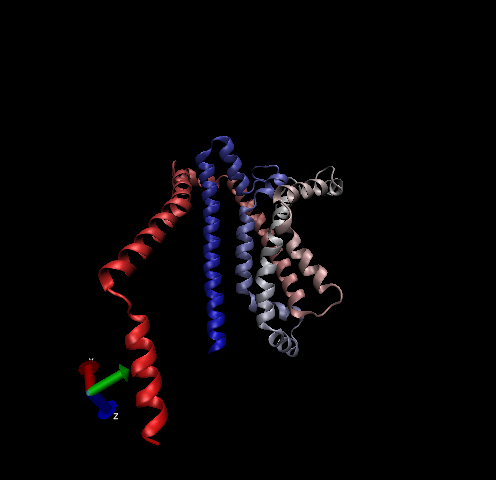
\includegraphics{predictedStructure.png}

\end{document}
